\documentclass[uplatex, titlepage]{jsarticle}
\usepackage[dvipdfmx]{graphicx}
\usepackage{float}


\title{通信の基礎02}
\author{C0118005 AM1 秋本 遥基}
\date{}

\begin{document}
\maketitle

\section{目的}

  静止画像のフォーマットの一つであるビットマップファイルについて情報量、色数、画素数のそれぞれに対して関係を調べる。PPMファイル、PNGファイルのファイルサイズとPNGファイルの画像圧縮が効果的な画像についてを比較し調べる。また、静止画像における周波数の概念を理解する。JPEG圧縮が人間の視覚特性を利用した圧縮方法であることを理解する。\\

\section{音の高さと周波数}
\label{sec:gazou}

\begin{figure}[H]
    \begin{tabular}{c}

      \begin{minipage}{0.3\hsize}
        \begin{center}
          \includegraphics[scale=0.3]{./myI/myImage24bit.bmp}
          \caption{24ビットビットマップ}
          \label{fig:24bitbitmap}
        \end{center}
      \end{minipage}
      \begin{minipage}{0.3\hsize}
        \begin{center}
          \includegraphics[scale=0.3]{./myI/myImage256.bmp}
          \caption{256色ビットマップ}
          \label{fig:256bitmap}
        \end{center}
      \end{minipage}
      \begin{minipage}{0.3\hsize}
        \begin{center}
          \includegraphics[scale=0.3]{./myI/myImage16.bmp}
          \caption{16色ビットマップ}
          \label{fig:16bitmap}
        \end{center}
      \end{minipage}

    \end{tabular}
\end{figure}

【結果】\\

  各画像のファイルサイズを以下の表\ref{table:bitfile}に示す。

\begin{table}[H]
  \centering
  \caption{ビットマップ形式とファイルサイズ}
  \label{table:bitfile}
  \begin{tabular}{|c|c|c|}\hline
    ファイル名 & ビットマップ形式名 & ファイルサイズ[バイト] \\ \hline
    myImage24bit.bmp & 24bit & 230454 \\ \hline
    myImage256.bmp & 256色 & 77878 \\ \hline
    myImage16.bmp & 16色 & 38518 \\ \hline
  \end{tabular}
\end{table}

\section{ビットマップファイルの構成(1)}

  \ref{sec:gazou}の中身を調べファイルサイズ、画像の幅、画像の幅、画像の高さ、色ビット数、画像データサイズを求める。\\

【結果】\\

  各画像について調べた結果を表\ref{table:zyoho24}から\ref{table:zyoho16}に示す。\\

\begin{table}[H]
  \centering
  \caption{ビットマップファイルからの情報の取得(myImage24bit.bmp)}
  \label{table:zyoho24}
  \begin{tabular}{|c|c|c|c|c|}\hline
     & データの位置[バイト目] & 16進表記(並び替え前) & 16進表記(並び替え後) & 10進表記 \\ \hline
     ファイルサイズ & $2~5$ & 36 84 03 00 & 00 03 84 36 & 230454 \\ \hline
     画像の幅 & 18~21 & 40 01 00 00 & 00 00 01 40 & 320 \\ \hline
     画像の高さ & 22~25 & f0 00 00 00 & 00 00 00 f0 & 240 \\ \hline
     色ビット数 & 28,29 & 18 00 & 00 18 & 24 \\ \hline
     画像データサイズ & 34~37 & 00 84 03 00 & 00 03 84 00 & 230400 \\ \hline
  \end{tabular}
\end{table}

\begin{table}[H]
  \centering
  \caption{ビットマップファイルからの情報の取得(myImage256.bmp)}
  \label{table:zyoho256}
  \begin{tabular}{|c|c|c|c|c|}\hline
     & データの位置[バイト目] & 16進表記(並び替え前) & 16進表記(並び替え後) & 10進表記 \\ \hline
     ファイルサイズ & 2~5 & 36 30 01 00 & 00 01 30 36 & 77878 \\ \hline
     画像の幅 & 18~21 & 40 01 00 00 & 00 00 01 40 & 320 \\ \hline
     画像の高さ & 22~25 & f0 00 00 00 & 00 00 00 f0 & 240 \\ \hline
     色ビット数 & 28,29 & 08 00 & 00 08 & 8 \\ \hline
     画像データサイズ & 34~37 & 00 2c 01 00 & 00 01 2c 00 & 76800 \\ \hline
  \end{tabular}
\end{table}

\begin{table}[H]
  \centering
  \caption{ビットマップファイルからの情報の取得(myImage16.bmp)}
  \label{table:zyoho16}
  \begin{tabular}{|c|c|c|c|c|}\hline
     & データの位置[バイト目] & 16進表記(並び替え前) & 16進表記(並び替え後) & 10進表記 \\ \hline
     ファイルサイズ & 2~5 & 76 96 00 00 & 00 00 96 76 & 38518 \\ \hline
     画像の幅 & 18~21 & 40 01 00 00 & 00 00 01 40 & 320 \\ \hline
     画像の高さ & 22~25 & f0 00 00 00 & 00 00 00 f0 & 240 \\ \hline
     色ビット数 & 28,29 & 04 00 & 00 04 & 4 \\ \hline
     画像データサイズ & 34~37 & 00 96 00 00 & 00 00 96 00 & 38400 \\ \hline
  \end{tabular}
\end{table}

\begin{table}[H]
  \centering
  \caption{色数}
  \label{table:irokazu}
  \begin{tabular}{|c|c|c|c|}\hline
    ファイル名 & 画像データサイズ[バイト] & N & 色数 \\ \hline
    myImage24bit.bmp & 230400 & 24 & 16777216   \\ \hline
    myImage256.bmp & 76800 & 8 & 256 \\ \hline
    myImage16.bmp & 38432 & 4 & 16 \\ \hline
  \end{tabular}
\end{table}

【考察】\\
(1) 比較すると、画像幅と高さが同一であるので画像に使用される色数が多くなるほどファイルサイズが大きくなる。\\
(2) 色ビット数が変わり、色数が少なくなったのでmyImage256.bmpとmyImage16.bmpがmyImage24bit.bmpより画質が悪くなった。\\
(3) ビット数Nは1ピクセルあたりに含まれる情報量であるから、画像データサイズを画素数で割ることにより求められる。\\

\section{ビットマップファイルの構成(2)}

  ビットマップファイルの中身を表示し、パレットデータ及び画像データの格納のされ方を確認する。また、ビットマップファイルと同様の色情報を持つPPM形式の画像ファイルの中身を確認し、同様であることを確認する。\\

【結果】\\

  結果を記入したものを以下図 に示す。\\


\begin{figure}[H]
    \begin{tabular}{c}

      \begin{minipage}{0.45\hsize}
        \begin{center}
          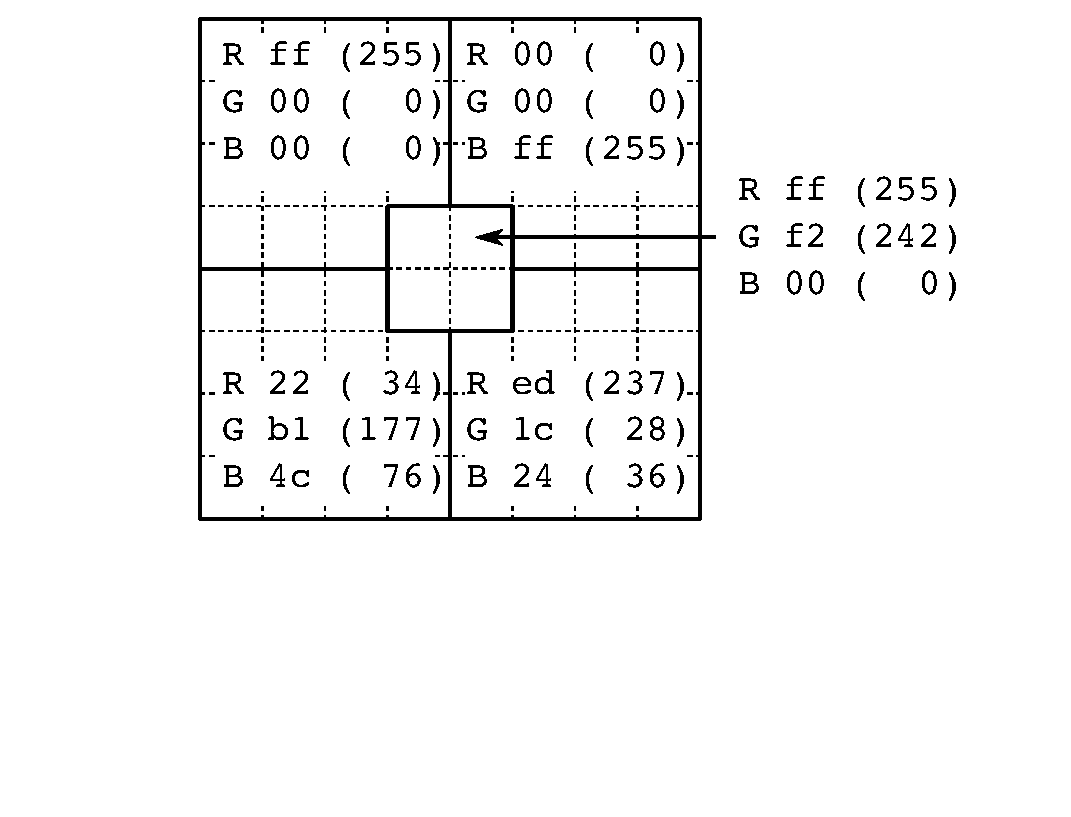
\includegraphics[scale=0.4]{./sikaku/8x8_24bitbmp.eps}
          \caption{画像データ(8x8\_24bit\.bmp)}
          \label{fig:24bitbmp}
        \end{center}
      \end{minipage}
      \begin{minipage}{0.45\hsize}
        \begin{center}
          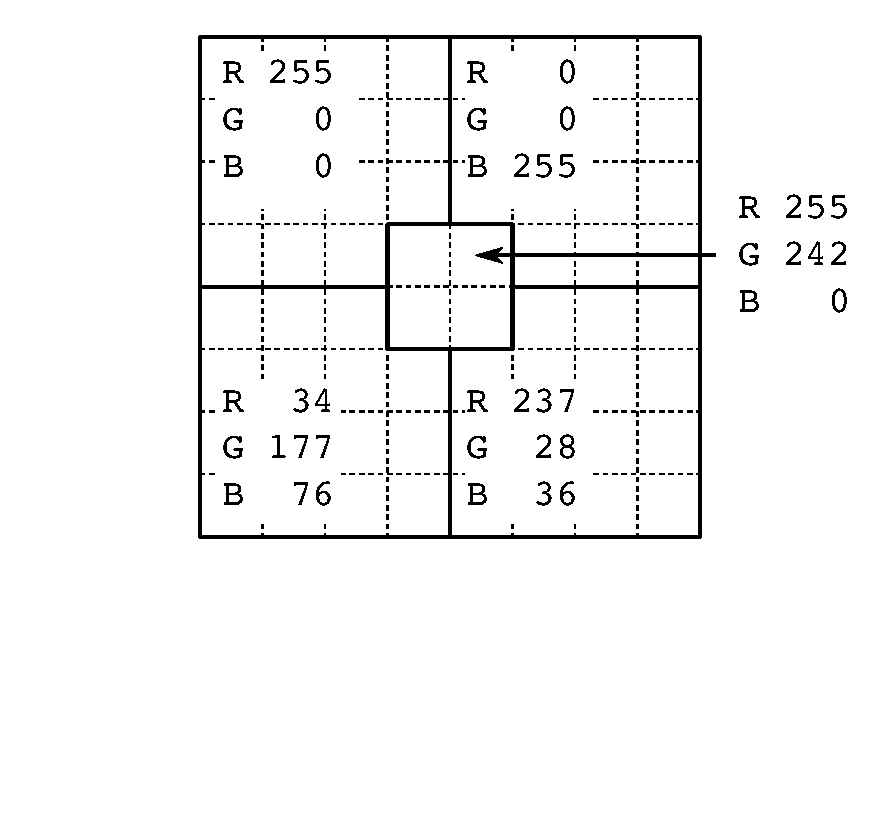
\includegraphics[scale=0.4]{./sikaku/8x8_24bitppm.eps}
          \caption{画像データ(8x8\_24bit\.ppm)}
          \label{fig:24bitppm}
        \end{center}
      \end{minipage}

    \end{tabular}
\end{figure}

\begin{figure}[H]
    \begin{tabular}{c}

      \begin{minipage}{0.45\hsize}
        \begin{center}
          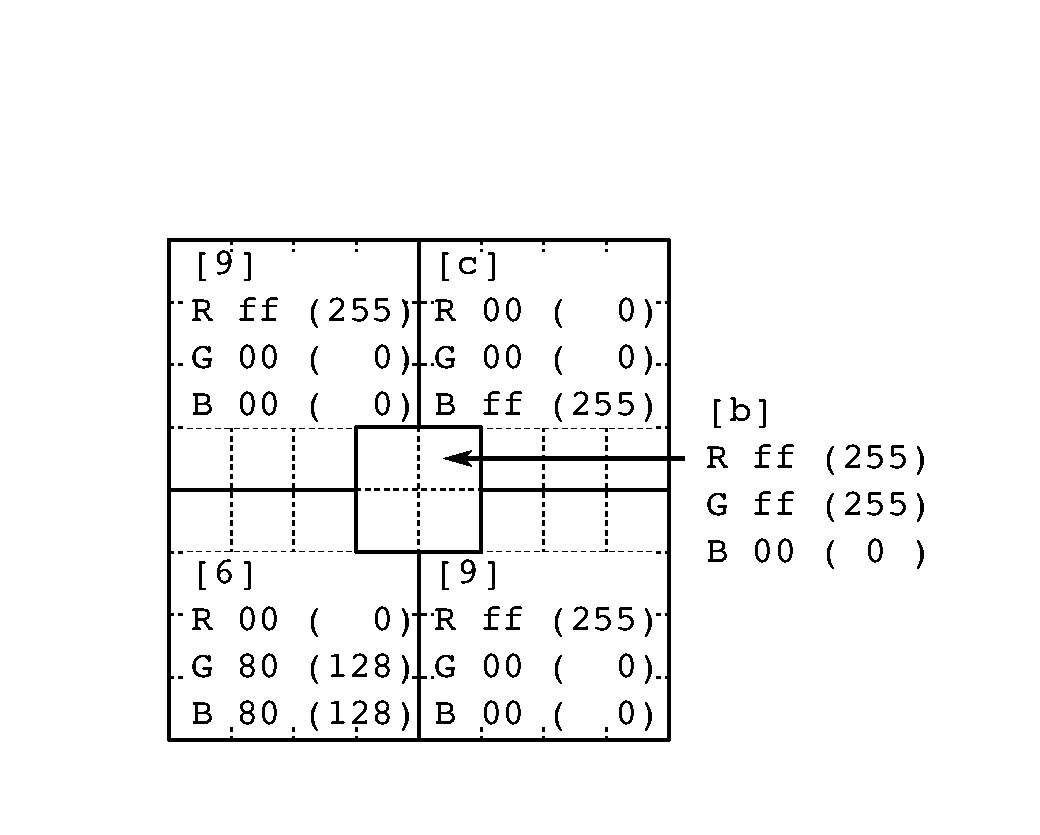
\includegraphics[scale=0.4]{./sikaku/8x8_16bmp.eps}
          \caption{画像データ(8x8\_16\.bmp)}
          \label{fig:16bmp}
        \end{center}
      \end{minipage}
      \begin{minipage}{0.45\hsize}
        \begin{center}
          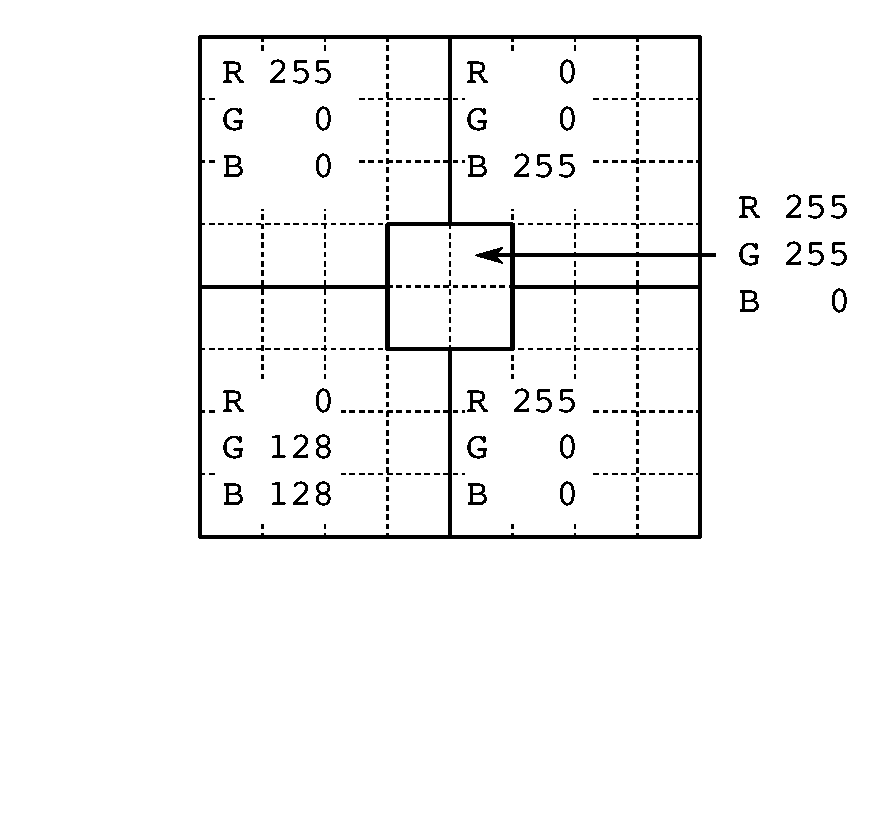
\includegraphics[scale=0.4]{./sikaku/8x8_16ppm.eps}
          \caption{画像データ(8x8\_16\.ppm)}
          \label{fig:16ppm}
        \end{center}
      \end{minipage}

    \end{tabular}
\end{figure}

\begin{figure}[H]
    \begin{tabular}{c}

      \begin{minipage}{0.45\hsize}
        \begin{center}
          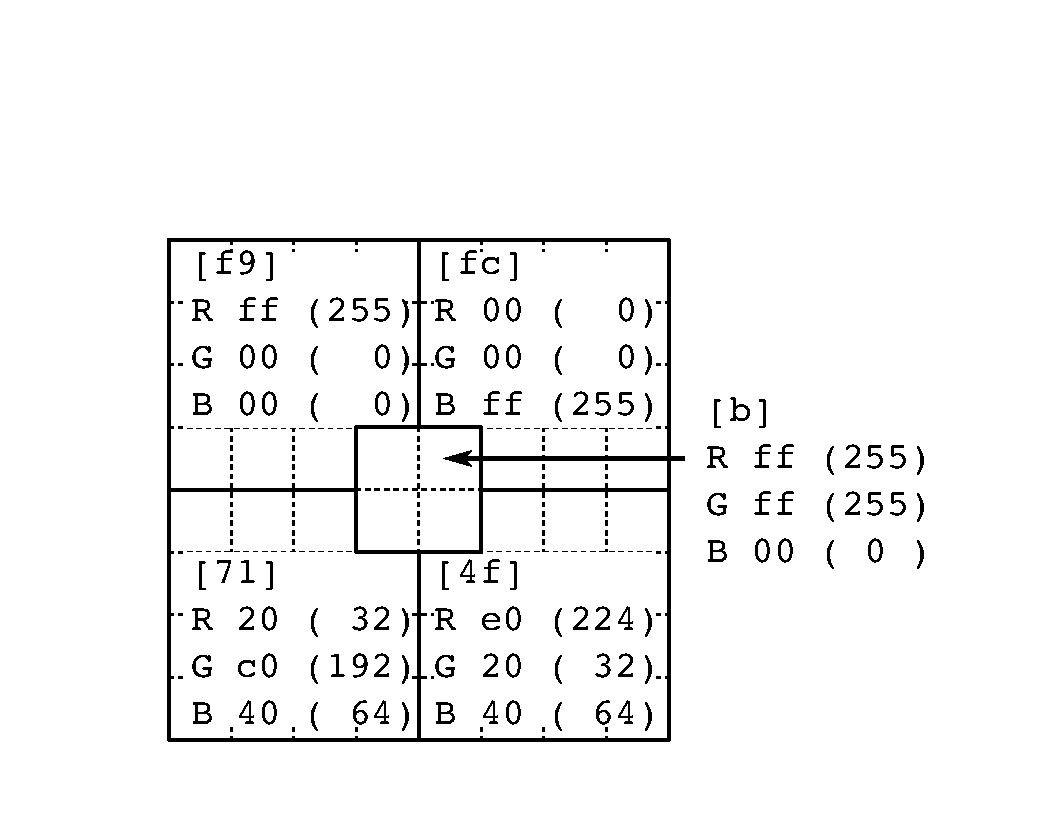
\includegraphics[scale=0.4]{./sikaku/8x8_256bmp.eps}
          \caption{画像データ(8x8\_256\.bmp)}
          \label{fig:256bmp}
        \end{center}
      \end{minipage}
      \begin{minipage}{0.45\hsize}
        \begin{center}
          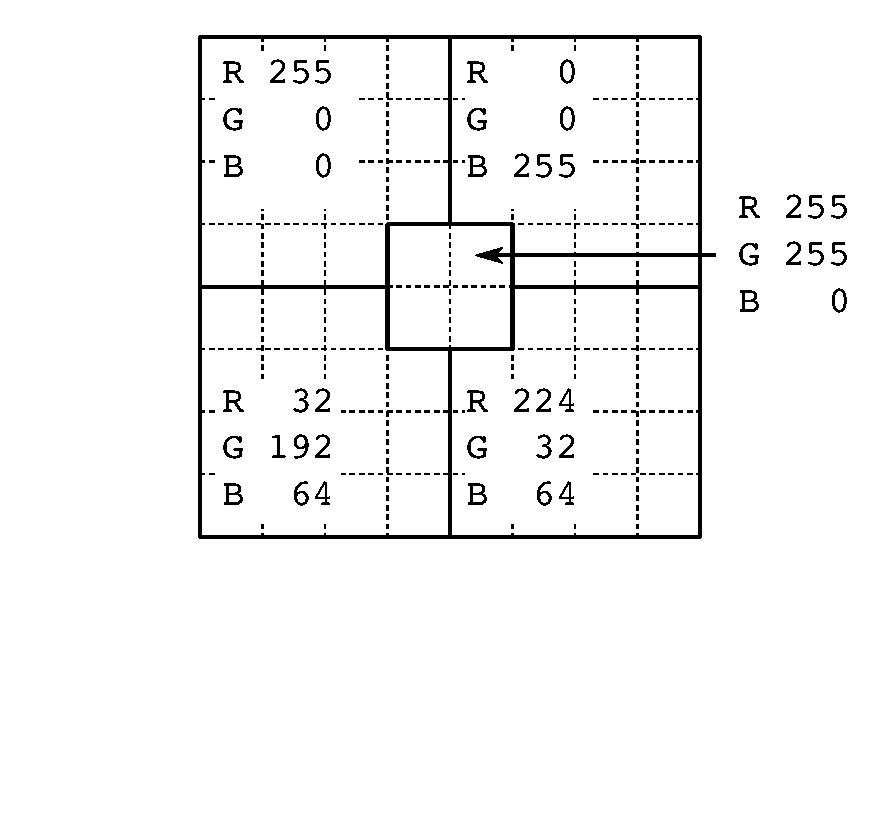
\includegraphics[scale=0.4]{./sikaku/8x8_256ppm.eps}
          \caption{画像データ(8x8\_256\.ppm)}
          \label{fig:256ppm}
        \end{center}
      \end{minipage}

    \end{tabular}
\end{figure}

【考察】\\

  16色ビットマップよりも256色ビットマップの方が色数が多いから元の表現に近い色味にするために画素が多く、それにより異なる画素が存在する。\\

\section{画像のフォーマットによるファイルサイズの違い}

  ビットマップ、PPM、PNGの画像フォーマットのそれぞれのフォーマットにおいてファイルサイズの違いを調べる。\\
【結果】\\
  結果を以下の\ref{table:tigai}に示す。
\begin{table}[H]
  \centering
  \caption{画像のフォーマットによるファイルサイズの違い}
  \label{table:tigai}
  \begin{tabular}{|c|c|c|c|} \hline
    ファイル名 & ビットマップ[バイト] & PPM[バイト] & PNG[バイト] \\ \hline
    marmot & 921654 & 921615 & 566816 \\ \hline
    cg & 921654 & 921615 & 101388 \\ \hline
    latticel & 921654 & 921615 & 372 \\ \hline
  \end{tabular}
\end{table}
【考察】\\
(1)画像サイズが各ファイルで同じかつビットマップ形式は非圧縮の画像形式であるから、3画像ともファイルサイズが同じである。\\
(2)PPM形式はビットマップ形式と同様に非圧縮の画像形式であるから、3画像ともファイルサイズが同じである。\\
(3)PNG形式は可逆圧縮の画像形式であるため、繰り返しの表現が可能な部分が多いものほど圧縮され、ファイルサイズが小さくなる。\\
(4)PNG形式の画像はビットマップ形式、PPM形式の画像と比べて、圧縮可能なファイル形式であるためファイルサイズが小さくなっている。\\

\section{画像によるPNGファイルのファイルサイズの違い}

  PNG画像を比較し、ファイルサイズの違いがどのような要因で生じたものか考察する。\\
【結果】\\
  結果を以下の表\ref{table:png}に示す。\\

\begin{table}[H]
  \centering
  \caption{画像によるPNGファイルのファイルサイズの違い}
  \label{table:png}
  \begin{tabular}{|c|c|} \hline
    ファイル名 & ファイルサイズ[バイト] \\ \hline
    lattice1.png & 372 \\ \hline
    lattice2.png & 695 \\ \hline
    lattice3.png & 602 \\ \hline
  \end{tabular}
\end{table}

【考察】\\
  PNG形式ではデフレート圧縮(LZ77とハフマン圧縮の組み合わせ)によって色数と、各色の繰り返しパターンによって圧縮される。
  したがって色数の少なさからlattice1が、パターンからlattice3がlattice2よりもサイズが小さくなる。\\

\section{8$ \times $8の画像の周波数と離散コサイン変換(DCT)}

  JPEGで空間周波数分析のために行われている離散コサイン変換(DCT)について、調べる。\\
【結果】\\
  結果を以下の表\ref{table:dct}に示す。\\

\begin{table}
  \centering
  \caption{係数の絶対値が最大となる(u,v)}
  \label{table:dct}
  \begin{tabular}{|c|c|c|} \hline
    \ & (u,v) & 周波数の低い順 \\ \hline
    白の塗りつぶし(8x8W.pgm) & (0,0) & 1 \\ \hline
    市松模様(8x8L.pgm) & (7,7) & 8 \\ \hline
    1ビット間隔の横縞(8x81bitB.pgm) & (7,0) & 7 \\ \hline
    1ビット間隔の縦縞(8x81bitS.pgm) & (0,7) & 6 \\ \hline
    2ビット間隔の横縞(8x82bitB.pgm) & (3,0) & 5 \\ \hline
    2ビット間隔の縦縞(8x82bitS.pgm) & (0,3) & 4 \\ \hline
    4ビット間隔の横縞(8x84bitB.pgm) & (1,0) & 3 \\ \hline
    4ビット間隔の縦縞(8x84bitS.pgm) & (0,1) & 2 \\ \hline
  \end{tabular}
\end{table}

【考察】\\
  画像の周波数は明るさと方向に基づいて決められる。
  したがってある範囲内でパターンが縦横に重複せず明暗が細かいほど高周波で、反対にパターンと明暗が一定のものが低周波となる。\\

\section{JPEGの品質と圧縮率}

  元画像から品質をそれぞれに変化させてJPEG画像を作成し、圧縮後のファイルサイズ及び圧縮率と劣化の具合を調べる。\\
【結果】\\
  結果を以下に示す。

\begin{table}
  \centering
  \caption{画像によるPNGファイルのファイルサイズの違い}
  \label{table:filesizemae}
  \begin{tabular}{|c|c|} \hline
    ファイル名 & ファイルサイズ[バイト] \\ \hline
    cg.bmp & 921654  \\ \hline
    marmot.bmp & 921654 \\ \hline
    wonbat.bmp & 921654 \\ \hline
    swiss.bmp & 921654 \\ \hline
  \end{tabular}
\end{table}

\begin{table}
  \centering
  \caption{圧縮後のファイルサイズ}
  \label{table:filesizeato}
  \begin{tabular}{|c|c|c|c|c|c|} \hline
    ファイル名 & \multicolumn{5}{|c|}{ファイルサイズ[バイト]} \\ \cline{2-6}
    (圧縮前) & 品質10\% & 品質30\% & 品質50\% & 品質70\% & 品質90\% \\ \hline
    cg.bmp & 10167 & 15626 & 19304 & 25306 & 38607  \\ \hline
    marmot.bmp & 14454 & 29703 & 41473 & 57383 & 108098 \\ \hline
    wonbat.bmp & 12442 & 24975 & 34443 & 47573 & 92194  \\ \hline
    swiss.bmp & 11902 & 22751 & 31410 & 43401 & 82454  \\ \hline
  \end{tabular}
\end{table}

\begin{table}
  \centering
  \caption{品質と圧縮率}
  \label{table:hinsituiasyuku}
  \begin{tabular}{|c|c|c|c|c|c|} \hline
    ファイル名 & \multicolumn{5}{|c|}{圧縮率[\%]} \\ \cline{2-6}
    (圧縮前) & 品質10\% & 品質30\% & 品質50\% & 品質70\% & 品質90\% \\ \hline
    cg.bmp & 1.10 & 1.70 & 2.09 & 2.75 & 4.19  \\ \hline
    marmot.bmp & 1.57 & 3.22 & 4.50 & 6.23 & 11.7 \\ \hline
    wonbat.bmp & 1.35 & 2.71 & 3.74 & 5.16 & 10.0  \\ \hline
    swiss.bmp & 1.29 & 2.47 & 3.41 & 4.71 & 8.95  \\ \hline
  \end{tabular}
\end{table}

\begin{figure}[H]
  \centering
  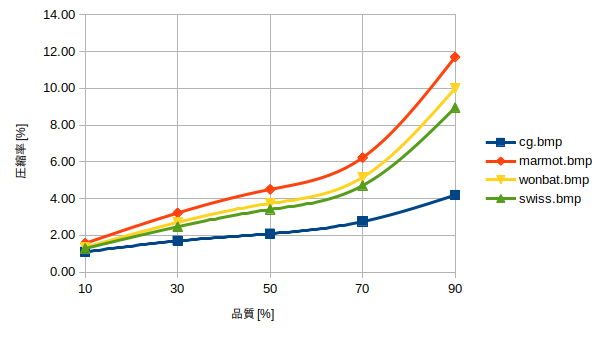
\includegraphics[scale=0.6]{./grahh.png}
  \caption{品質と圧縮率の関係}
  \label{fig:hinsitu}
\end{figure}

\begin{table}
  \centering
  \caption{画像の劣化}
  \label{table:gazourekka}
  \begin{tabular}{|c|c|c|c|} \hline
    ファイル名 & 品質[\%] & 劣化の具合 & PSNR[dB] \\ \hline
    cg.bmp & 90 &  & 41.9   \\ \cline{2-4}
     & 70 & 文字周辺にノイズ、背景にノイズ & 37.5   \\ \cline{2-4}
     & 50 & 上記と同様 & 35.3   \\ \cline{2-4}
     & 30 & 上記と同様 & 33.1   \\ \cline{2-4}
     & 10 & 上記と同様 & 28.2   \\ \hline%cline{2-4}
    marmot.bmp & 90 &  & 32.9 \\ \cline{2-4}%hline
     & 70 & ごく僅かにノイズ & 29.2   \\ \cline{2-4}
     & 50 & 少量のノイズ & 27.7   \\ \cline{2-4}
     & 30 & 全体にノイズ & 26.4   \\ \cline{2-4}
     & 10 & 全体に多量のノイズ & 23.8   \\ \hline%cline{2-4}
    wonbat.bmp & 90 &  & 37.3  \\ \cline{2-4}%\hline
     & 70 &  & 33.5   \\ \cline{2-4}
     & 50 &  & 32.0   \\ \cline{2-4}
     & 30 & 毛の部分にかすかにノイズ & 30.6   \\ \cline{2-4}
     & 10 & 全体にノイズ & 27.2   \\ \hline%cline{2-4}
    swiss.bmp & 90 &  & 36.1   \\ \cline{2-4}%\hline
     & 70 &  & 32.4   \\ \cline{2-4}
     & 50 & 全体にノイズ & 31.0   \\ \cline{2-4}
     & 30 & 上記と同様 & 29.6   \\ \cline{2-4}
     & 10 & 上記と同様 & 26.4   \\ \hline
  \end{tabular}
\end{table}

【考察】\\
  表\ref{table:hinsituiasyuku}より、cg.bmp、swiss.bmp、wonbat.bmp、marmot.bmpの順に圧縮率が低かった。
  したがって色の変化の激しさによって圧縮率に差が出るように思われる。\\

\section{JPEGにおける量子化テーブル}

  決められたステップサイズ別にファイルを圧縮し、ファイルサイズや画質がどのように変化するか調べる。\\
【結果】\\
  以下に結果を示す。\\

\begin{table}
  \centering
  \caption{ステップサイズと圧縮率}
  \label{table:stepasyuku}
  \begin{tabular}{|c|c|c|} \hline
    & ビットマップ[バイト] & 圧縮率[\%] \\ \hline
    圧縮率 & 921654 & - \\ \hline
    ステップサイズ 32 & 43455 & 4.71 \\ \hline
    ステップサイズ 64 & 25612 & 2.78 \\ \hline
    ステップサイズ 96 & 17857 & 1.94 \\ \hline
    ステップサイズ 128 & 13911 & 1.51 \\ \hline
  \end{tabular}
\end{table}

\begin{figure}[H]
  \centering
  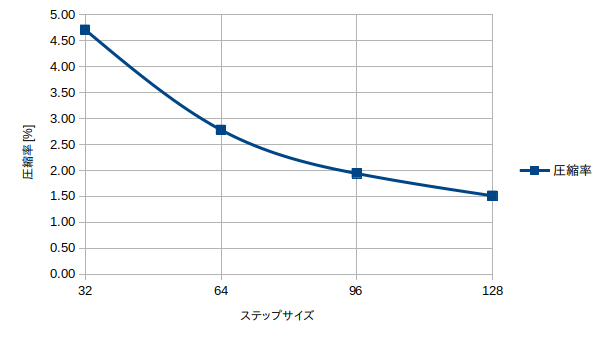
\includegraphics[scale=0.6]{./grahh2.png}
  \caption{ステップサイズと圧縮率の関係}
  \label{fig:step}
\end{figure}

\begin{table}[H]
  \centering
  \caption{ステップサイズによる画像の劣化の違い}
  \label{table:steprekka}
  \begin{tabular}{|c|c|c|} \hline
    ステップサイズ & 劣化の具合 & PSNR[dB] \\ \hline
    32 & 背景に少量のノイズ & 28.5 \\ \hline
    64 & 背景全体にノイズ & 26.0 \\ \hline
    96 & 背景とマーケットにノイズ & 24.4 \\ \hline
    128 & 下部の草以外に酷いノイズ & 23.4 \\ \hline
  \end{tabular}
\end{table}

\begin{table}[H]
  \centering
  \caption{圧縮する条件による画像の劣化の違い}
  \label{table:zyoukenrekka}
  \begin{tabular}{|c|c|c|c|} \hline
     & 条件 & ファイルサイズ[バイト] & 劣化の具合 \\ \hline
    d) & A 64 & 19075 & 背景とマーモットにノイズ   \\ %\cline{2-4}
     & それ以外 128 &  &    \\ %\cline{2-4}
     &  &  &    \\ %\cline{2-4}
     &  &  &    \\ \hline
    d) & B 49 & 18877 & 草以外極めて酷いノイズ   \\ %\cline{2-4}
     & それ以外 128 &  &    \\ %\cline{2-4}
     &  &  &    \\ %\cline{2-4}
     &  &  &    \\ \hline
  \end{tabular}
\end{table}

  図\ref{fig:step}より、ステップサイズの大きい高周波がより圧縮される。\\

【考察】\\
(1)図5.3でのAは64,それ以外は128のステップサイズとなっている。 \\
  したがってAの部分は、 \\
\begin{equation}
  256 / 64 = 4 = 2^2
\end{equation}
  よって、2bitであり、A以外の部分は、 \\
\begin{equation}
  256 / 128 = 2 = 2^1
\end{equation}
  よって、1bitである。 \\
(2)表\ref{table:zyoukenrekka}のd)は高周波成分が、e)は低周波成分がより圧縮されやすくなっている。ファイルサイズが同じ程度の場合には、高周波成分を圧縮したほうが画像の劣化が抑えられる。 \\


\begin{thebibliography}{99}
  \bibitem{one} \verb+"静止画像の構成(JPEG),https://service.cloud.teu.ac.jp/lecture/CSF/kinoshi/%E9%80+
  \verb+%9A%E4%BF%A1%E3%81%AE%E5%9F%BA%E7%A4%8E/5.Image(JPEG).pdf+
  (参照:\today)
  \end{thebibliography}
\end{document}






























\begin{table}
  \centering
  \caption{画像のフォーマットによるファイルサイズの違い}
  \label{}
  \begin{tabular}{|c|c|c|c|} \hline
    ファイル名 & ビットマップ[バイト] & PPM[バイト] & PNG[バイト] \\ \hline
    marmot & x & y & z \\ \hline
    cg & x & y & z \\ \hline
    latticel & x & y & z \\ \hline
  \end{tabular}
\end{table}

%
\begin{figure}[H]
    \begin{tabular}{c}

      \begin{minipage}{0.45\hsize}
        \begin{center}
          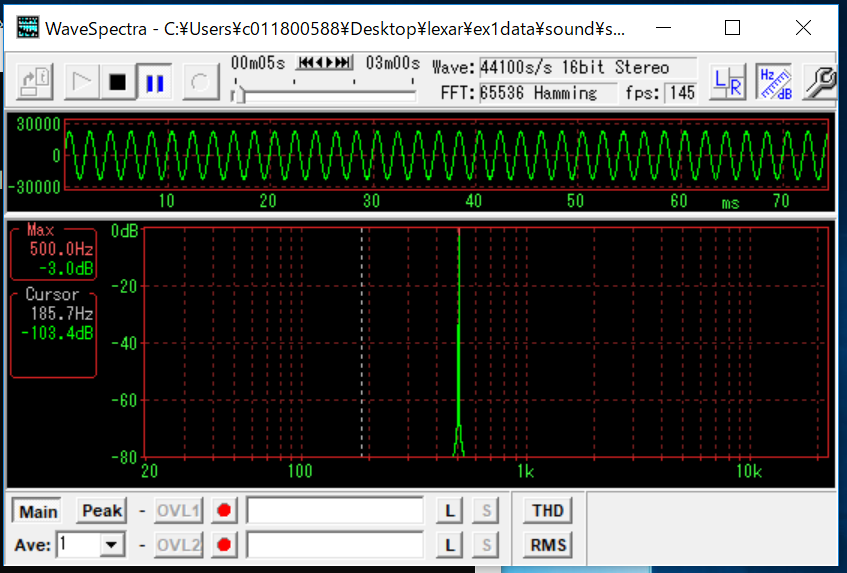
\includegraphics[scale=0.45]{./tuusin1.2/sin.png}
          \caption{500[Hz] サイン波}
          \label{fig:sin}
        \end{center}
      \end{minipage}

      \begin{minipage}{0.45\hsize}
        \begin{center}
          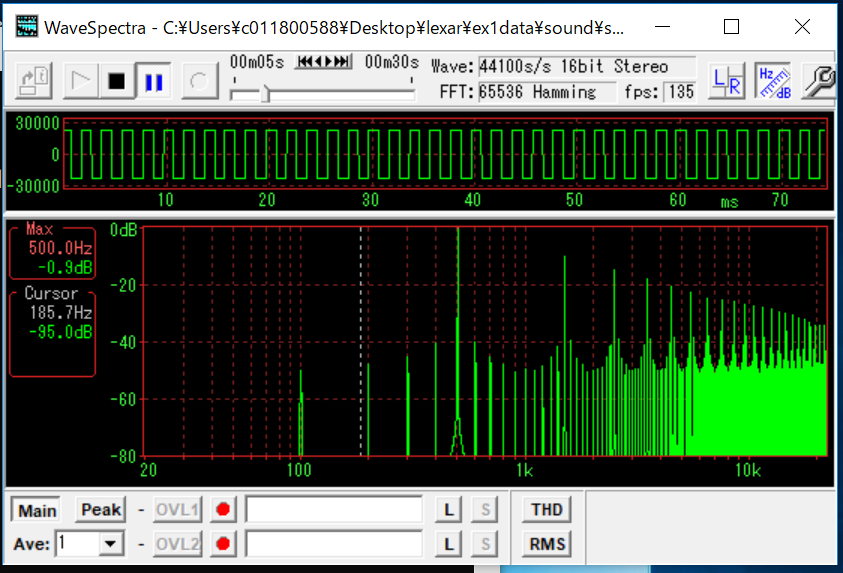
\includegraphics[scale=0.45]{./tuusin1.2/square500.png}
          \caption{500[Hz] 矩形波}
          \label{fig:squ}
        \end{center}
      \end{minipage}

    \end{tabular}
\end{figure}


\begin{figure}[H]
  \centering
  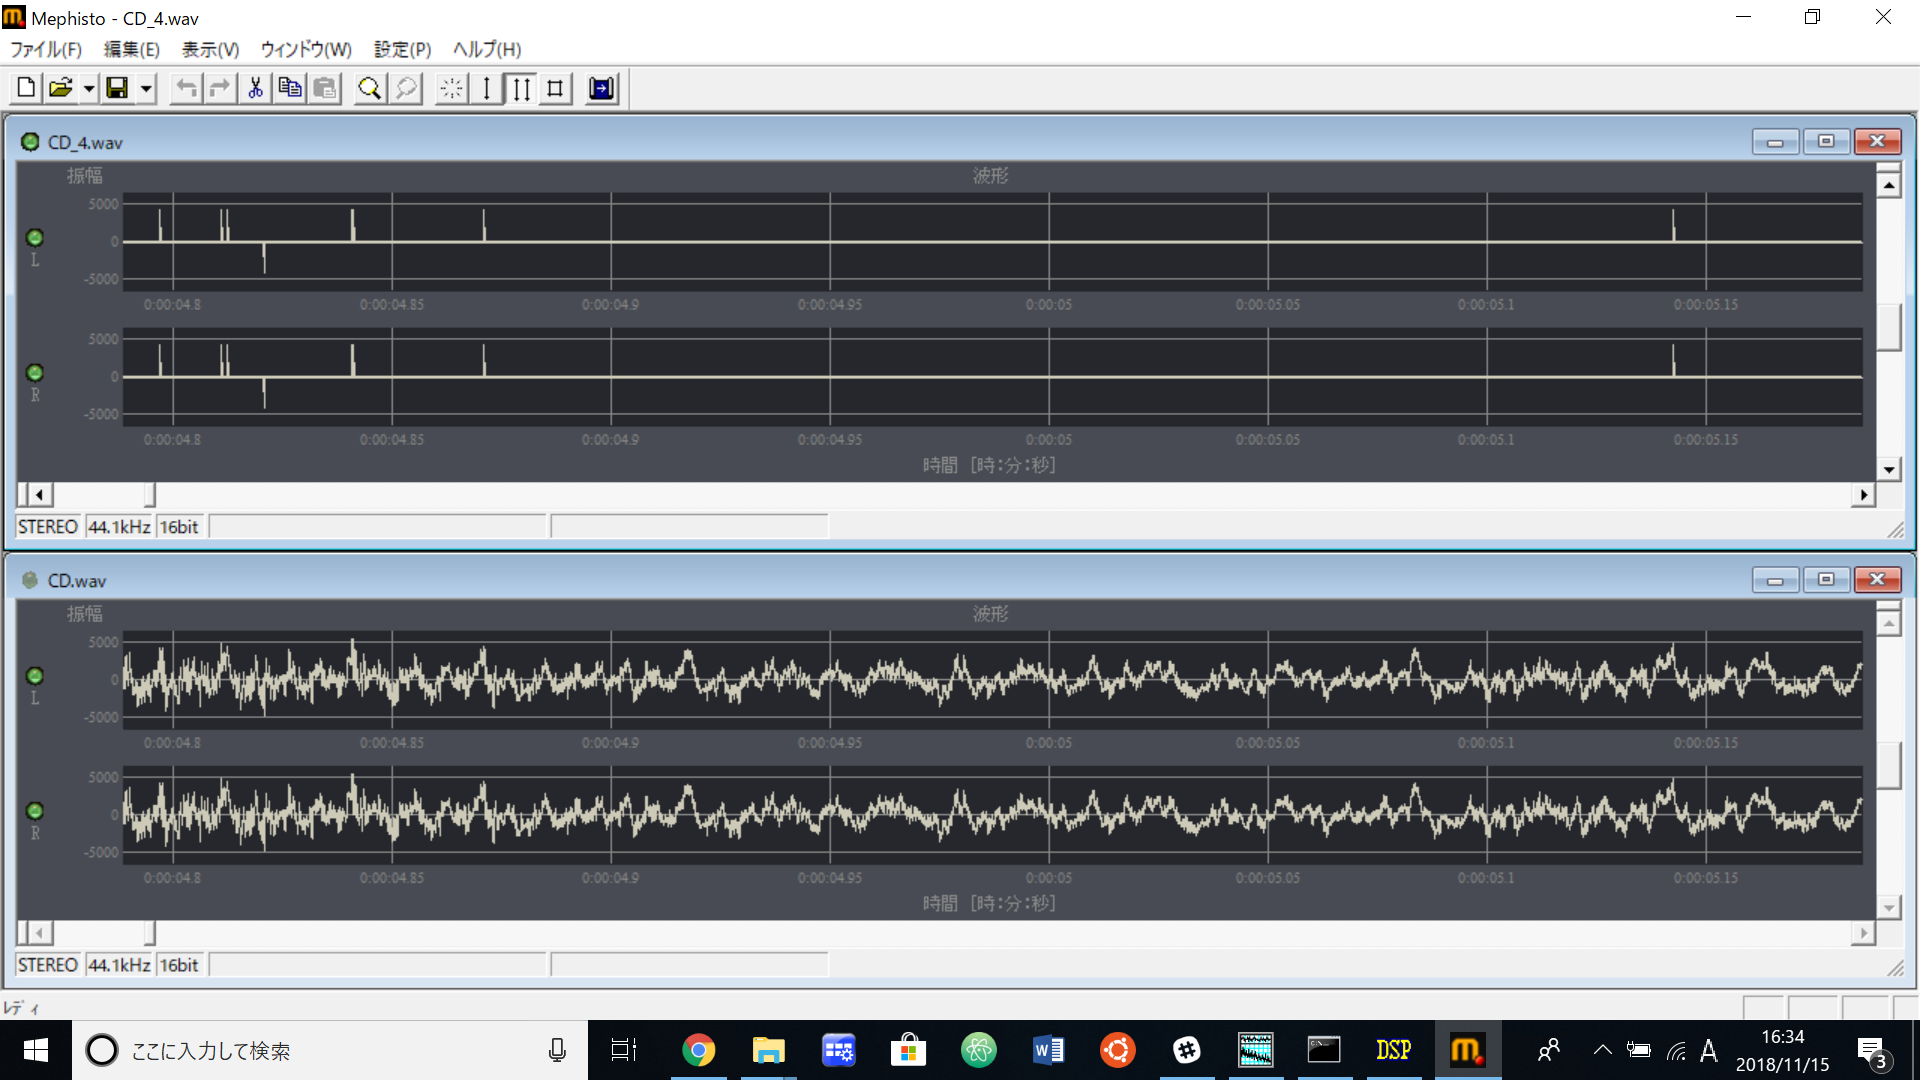
\includegraphics[scale=0.4]{./tuusin1.4/diff4.png}
  \caption{オリジナル波形と量子化ビット数4bitの波形}
  \label{fig:4bit}
\end{figure}


\begin{thebibliography}{99}
  \bibitem{one} \verb+"音の性質とサンプリング、量子化",https://service.cloud.teu.ac.jp/lecture/CSF+
  \verb+/kinoshi/%E9%80%9A%E4%BF%A1%E3%81%AE%E5%9F%BA%E7%A4%8E/1.Sound(Sampling,Quantization).pdf,+
  (参照:\today)
  \end{thebibliography}
\end{document}
